\documentclass[14pt]{extreport}
\usepackage{cmap}
\usepackage[utf8]{inputenc}
\usepackage[english,ukrainian]{babel}
\usepackage{graphicx}
\usepackage{geometry}
\usepackage{listings}
\usepackage{amsmath}
\usepackage{float}
\geometry{
	a4paper,
	left=20mm,
	right=20mm,
	top=20mm,
	bottom=20mm
}
\lstset{
	columns=fullflexible, 
	frame=single, 
	breaklines=true, 
	tabsize=4,
	postbreak=\raisebox{0ex}[0ex][0ex]{\ensuremath{\hookrightarrow\space}},
	showstringspaces=false,% no symbol for spaces in strings
}
\graphicspath{ {./pictures} }
\setlength{\parindent}{4em}

\newcommand\subject{Бази даних}
\newcommand\lecturer{асистент кафедри ПЗ\\Білоіваненко М.В.}
\newcommand\teacher{асистент кафедри ПЗ\\Білоіваненко М.В.}
\newcommand\mygroup{ПЗ-32}
\newcommand\lab{7}
\newcommand\theme{Індекси у плані виконання запитів}
\newcommand\purpose{Обрати типові запити на вибірку. Проаналізувати їхні плани виконання із різними операторами порівняння значень. Проаналізувати структуру плану виконання запиту, що містить декілька з’єднань таблиць. Встановити таблиці, які будуть мати постійний приріст даних при експлуатації}

\begin{document}
\begin{normalsize}
	\begin{titlepage}
		\thispagestyle{empty}
		\begin{center}
			\textbf{МІНІСТЕРСТВО ОСВІТИ І НАУКИ УКРАЇНИ\\
				НАЦІОНАЛЬНИЙ УНІВЕРСИТЕТ "ЛЬВІВСЬКА ПОЛІТЕХНІКА"}
		\end{center}
		\begin{flushright}
			Інститут \textbf{КНІТ}\\
			Кафедра \textbf{ПЗ}
		\end{flushright}
		\vspace{200pt}
		\begin{center}
			\textbf{ЗВІТ}\\
			\vspace{10pt}
			До лабораторної роботи № \lab\\
			\textbf{На тему}: “\textit{\theme}”\\
			\textbf{З дисципліни}: “\subject”
		\end{center}
		\vspace{40pt}
		\begin{flushright}
			
			\textbf{Лектор}:\\
			\lecturer\\
			\vspace{10pt}
			\textbf{Виконав}:\\
			
			студент групи \mygroup\\
			Коваленко Д.М.\\
			\vspace{10pt}
			\textbf{Прийняв}:\\
			
			\teacher\\
			
			\vspace{28pt}
			«\rule{1cm}{0.15mm}» \rule{1.5cm}{0.15mm} 2023 р.\\
			$\sum$ = \rule{1cm}{0.15mm}……………\\
			
		\end{flushright}
		\vspace{\fill}
		\begin{center}
			\textbf{Львів — 2023}
		\end{center}
	\end{titlepage}
		
	\begin{description}
		\item[Тема.] \theme.
		\item[Мета.] \purpose.
	\end{description}

	\section*{Лабораторне завдання}
	Обрати типові запити на вибірку. Проаналізувати їхні плани виконання із різними операторами порівняння значень. Проаналізувати структуру плану виконання запиту, що містить декілька з’єднань таблиць. Встановити таблиці, які будуть мати постійний приріст даних при експлуатації
	
	\begin{enumerate}
\item Додати індекси до колонок із зовнішніми ключами, якщо це не зроблено СУБД автоматично.
\item Додати комплексний індекс та індекс на функцію, встановити факт їх використання за планом виконання.
\item Додати 3 індекси на важливі колонки для підвищення ефективності запитів.
	\end{enumerate}
	
	\section*{Хід роботи}
	
	Створення індексів до колонок із зовнішніми ключами.
	\begin{small}
		\begin{lstlisting}[language=sql]
create index idx_driver_route_driver_id on driver_route (driver_id);
create index idx_driver_route_vehicle_id on driver_route (vehicle_id);
create index idx_driver_route_route_id on driver_route (route_id);
create index idx_route_first_stop_id on route (first_stop_id);
create index idx_route_last_stop_id on route (last_stop_id);
create index idx_route_stop_route_id on route_stop (route_id);
create index idx_route_stop_stop_id on route_stop (stop_id);
create index idx_ticket_route_id on ticket (route_id);
create index idx_ticket_vehicle_id on ticket (vehicle_id);
create index idx_schedule_vehicle_id on schedule (vehicle_id);
create index idx_schedule_route_id on schedule (route_id);
create index idx_schedule_stop_id on schedule (stop_id);
create index idx_vehicle_maintenance_vehicle_id on vehicle_maintenance (vehicle_id);
		\end{lstlisting}
	\end{small}

	\begin{figure}[H]
		\centering
		\includegraphics[scale=0.38]{5}
		\caption{План виконання складного запиту до створення індексів на зовнішні ключі.}
	\end{figure}
	
	\begin{figure}[H]
		\centering
		\includegraphics[scale=0.35]{6}
		\caption{План виконання складного запиту після створення індексів на зовнішні ключі.}
	\end{figure}
	
	Створення комплексного індексу та індексу на функцію.
	\begin{small}
		\begin{lstlisting}[language=sql]
create index idx_ticket_route_id_vehicle_id on ticket (route_id, vehicle_id)
create index idx_ticket_fare_amount on ticket ((fare * amount));
		\end{lstlisting}
	\end{small}
	
	\begin{figure}[H]
		\centering
		\includegraphics[scale=0.7]{1}
		\caption{План виконання до створення комплексного індекса на колонки.}
	\end{figure}
	
	\begin{figure}[H]
		\centering
		\includegraphics[scale=0.5]{2}
		\caption{План виконання після створення комплексного індекса на колонки.}
	\end{figure}
	
	\begin{figure}[H]
		\centering
		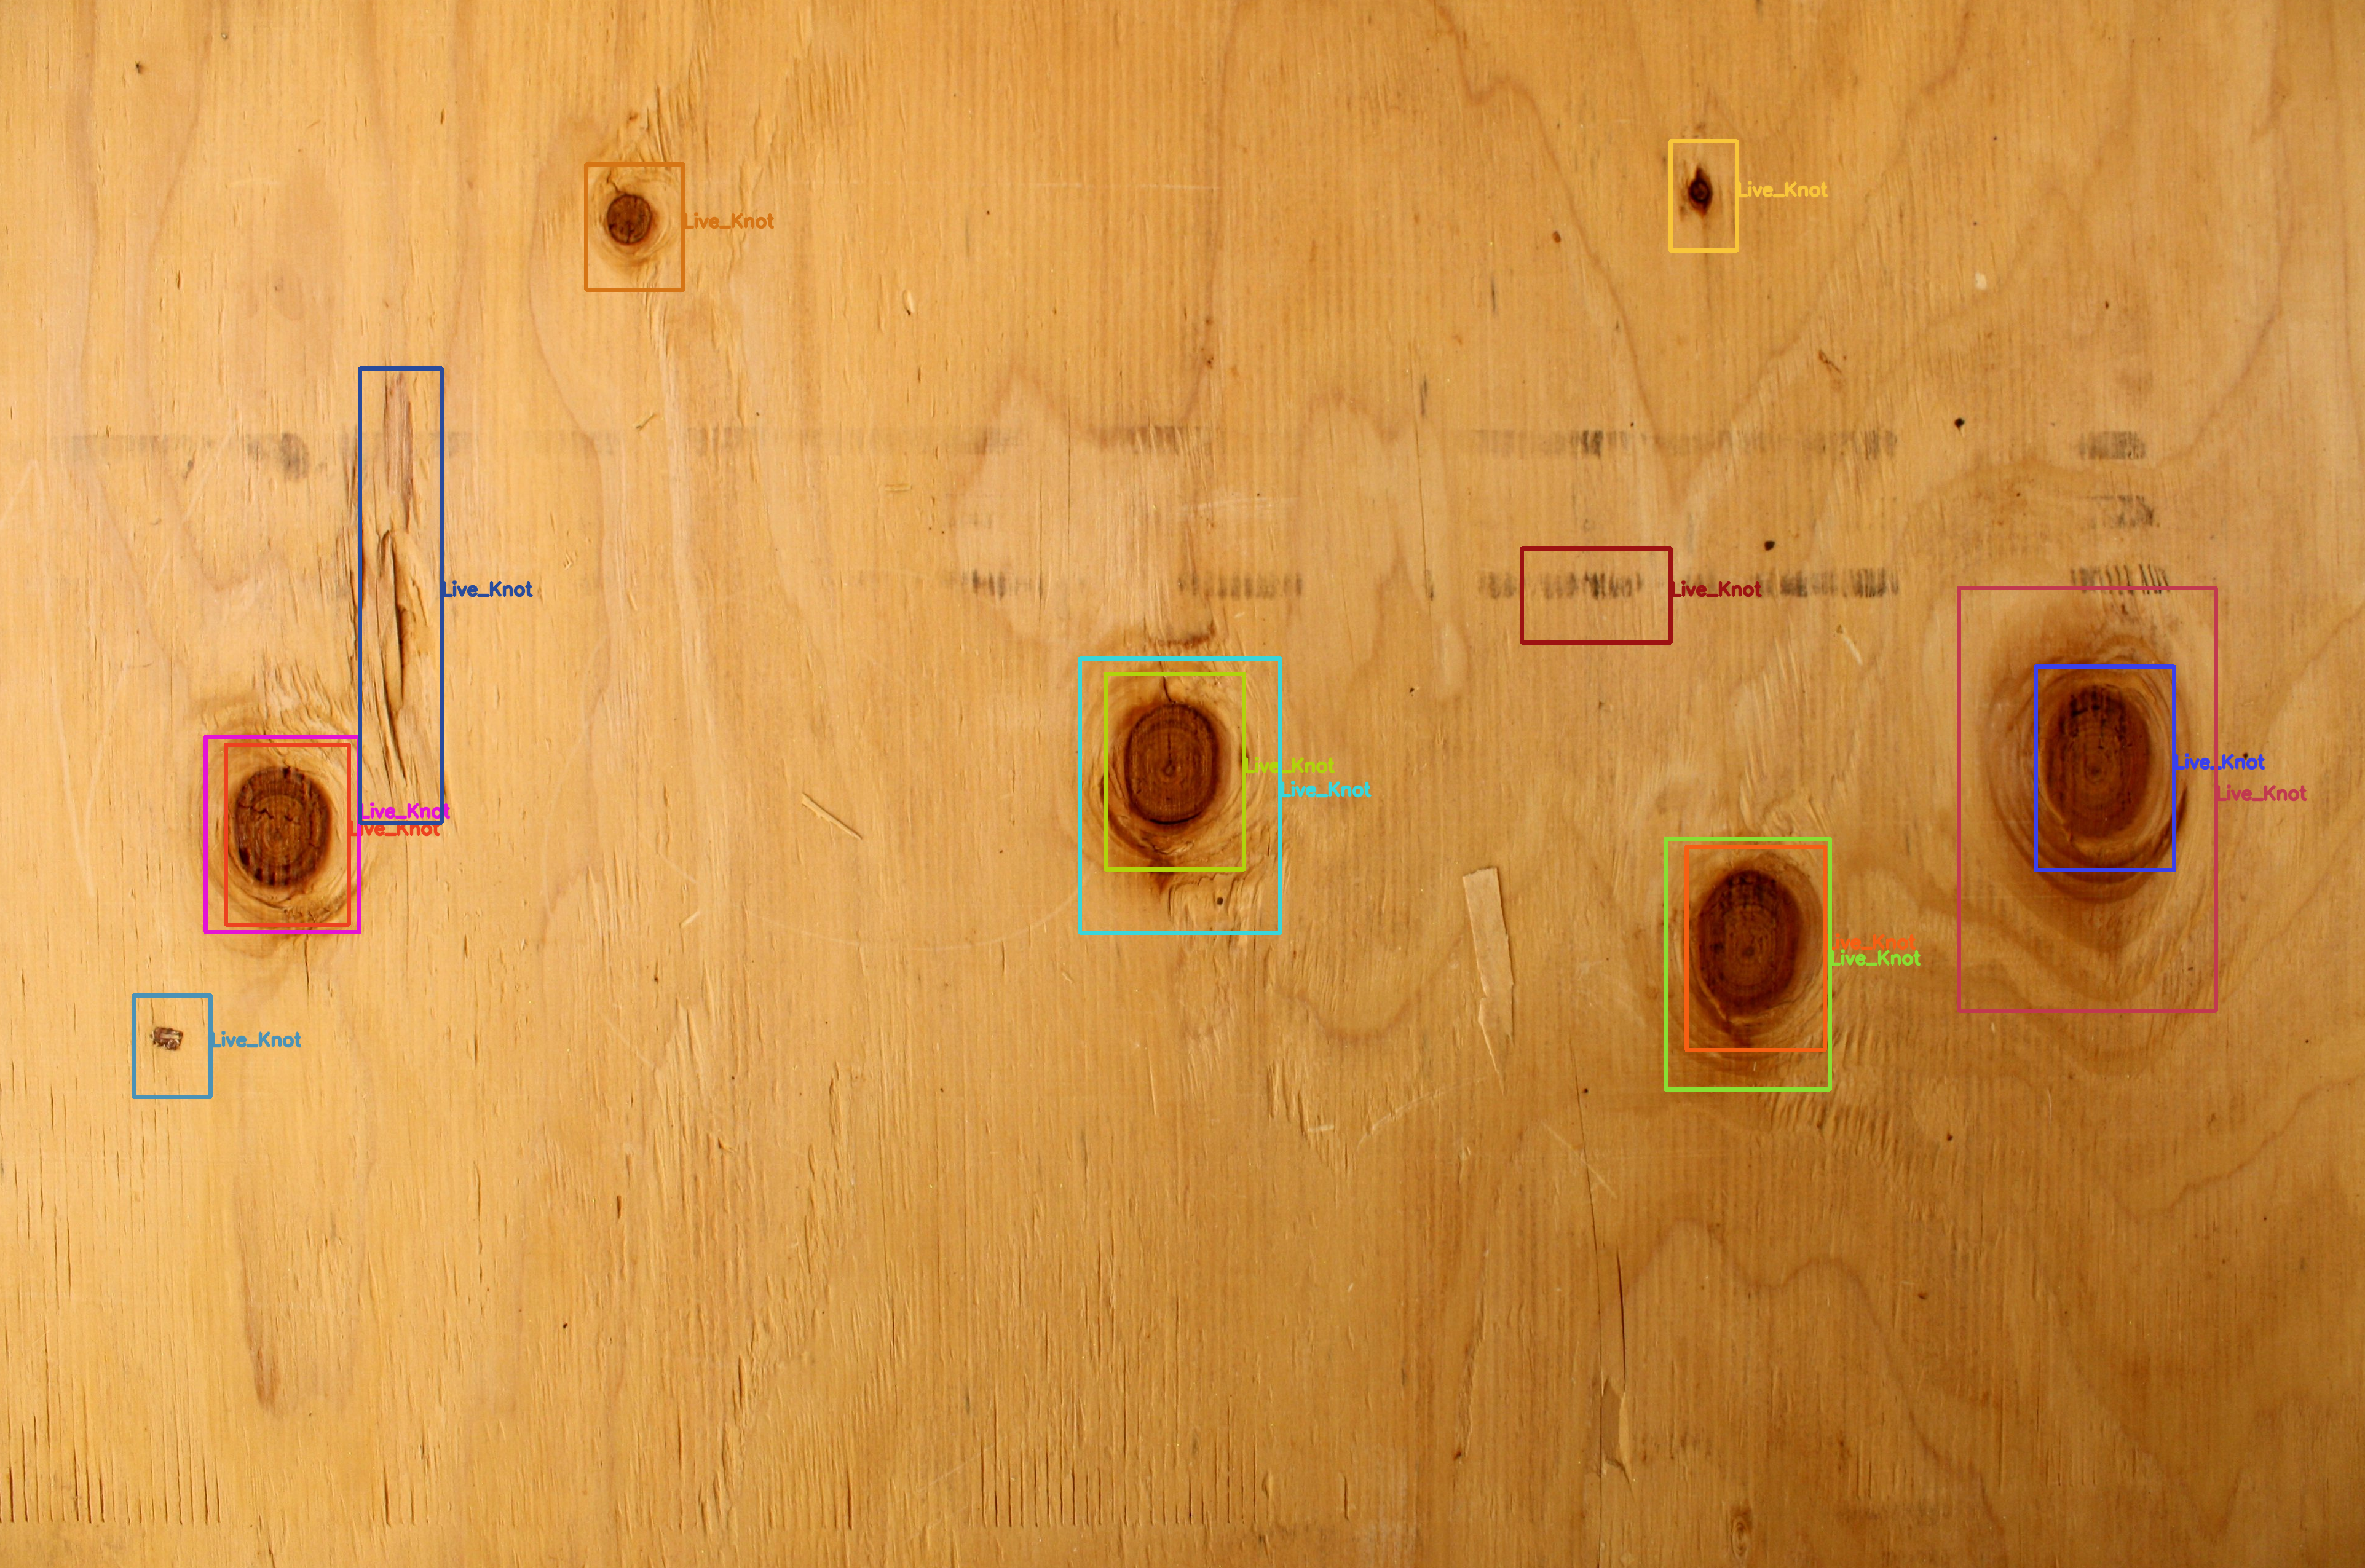
\includegraphics[scale=0.65]{3}
		\caption{План виконання до створення комплексного індекса на функцію.}
	\end{figure}
	
	\begin{figure}[H]
		\centering
		\includegraphics[scale=0.55]{4}
		\caption{План виконання після створення комплексного індекса на функцію.}
	\end{figure}
	Створення 3х індексів на важливі колонки для підвищення ефективності запитів.
	\begin{small}
		\begin{lstlisting}[language=sql]
create index idx_driver_first_name on driver (first_name);
create index idx_route_name on route (name);
create index idx_vehicle_license_plate on vehicle (license_plate);
		\end{lstlisting}
	\end{small}
	
	\section*{Висновок}
	Під час виконання лабораторної роботи я обрав типові запити на вибірку. Проаналізував їхні плани виконання із різними операторами порівняння значень. Проаналізував структуру плану виконання запиту, що містить декілька з’єднань таблиць. Встановив таблиці, які будуть мати постійний приріст даних при експлуатації.
	 
\end{normalsize}
\end{document}
